\label{ch:eda}
\section{Objectives and Method}
\label{sec:eda-objectives}

Before trusting any neural summarizer or citation verifier, this thesis asks what Multi-LexSum \emph{actually} contains. The exploratory data analysis (EDA) is implemented in \texttt{notebooks/multilexsum\_eda.ipynb} and writes reproducible tables to \texttt{code/reports/tables/} and figures to \texttt{Documentation/figures/eda/}. The analysis addresses five practical questions:
\begin{enumerate}
  \item How are cases distributed across splits, and which summary granularities are available per case?
  \item How do expert summary lengths compare to the paper's target word counts?
  \item How long and heterogeneous are multi-document sources, and what fraction exceeds common model context budgets?
  \item What civil-rights case types and filing years does the benchmark cover?
  \item How densely do expert summaries contain case-citation patterns at each granularity, motivating the symbolic verification module?
\end{enumerate}

All statistics below are computed on \textbf{4{,}539 cases} (train: 3{,}177; validation: 454; test: 908), matching the Hugging Face release structure of one row per case with up to three summary fields. Each figure is interpreted in three steps: \emph{what it shows}, \emph{what it implies}, and \emph{how it changes system design}.

\section{Corpus Shape and Summary Availability}
\label{sec:eda-corpus-shape}

Table~\ref{tab:split-inventory} confirms the standard Multi-LexSum split sizes. Unlike the paper's count of 9{,}280 \emph{summary instances}, the released dataset stores one record per case; long summaries are present for every case, while short and tiny summaries are partially missing.

\begin{table}[!t]
\centering
\caption{Multi-LexSum split inventory (cases per split).}
\label{tab:split-inventory}
\begin{tabular}{@{}l r@{}}
\toprule
\textbf{Split} & \textbf{Cases} \\
\midrule
Train      & 3{,}177 \\
Validation & 454 \\
Test       & 908 \\
\midrule
\textbf{Total} & \textbf{4{,}539} \\
\bottomrule
\end{tabular}
\end{table}

Long summaries (\texttt{summary/long}) are present for 100\% of cases in every split. Short summaries are present for 69.6\% (train), 68.7\% (validation), and 67.8\% (test). Tiny summaries are present for only 35.6\%, 35.5\%, and 34.4\%, respectively.

\begin{figure}[!t]
\centering
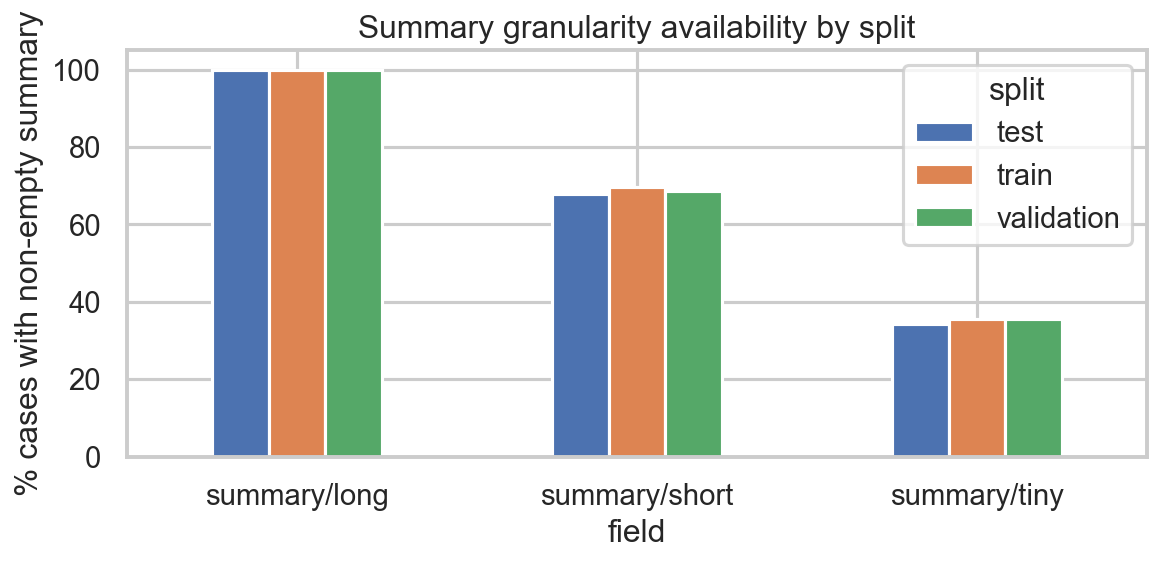
\includegraphics[width=0.92\linewidth]{summary_availability.png}
\caption{Percentage of cases with a non-empty expert summary at each granularity, by split. Long summaries form a complete bar at 100\%; short and tiny bars fall substantially lower.}
\label{fig:summary-availability}
\end{figure}

\paragraph{Reading Figure~\ref{fig:summary-availability}.}
The plot compares three granularities across train/validation/test. The dominant visual signal is the unbroken 100\% availability of long summaries contrasted with partial short coverage and sparse tiny coverage. The pattern is stable across splits, which indicates a dataset design property rather than a split-specific corruption.

\paragraph{Design implication.}
Tasks $D\rightarrow S$ and especially $D\rightarrow T$ have fewer supervised targets than $D\rightarrow L$. Primary summarization and citation-verification experiments therefore prioritize document-to-long summarization.

\section{Summary Length Distributions}
\label{sec:eda-summary-lengths}

Table~\ref{tab:summary-word-stats} compares empirical word-count statistics on the test split to the paper's target averages (650 / 130 / 25 words). Median long-summary length (407 words) is below the 650-word target but within the same order of magnitude; short and tiny medians (97 and 19 words) track the paper targets closely.

\begin{table}[!t]
\centering
\caption{Expert summary word-count statistics on the test split (present summaries only).}
\label{tab:summary-word-stats}
\begin{tabular}{@{}l r r r r@{}}
\toprule
\textbf{Field} & \textbf{$n$} & \textbf{Mean} & \textbf{Median} & \textbf{Paper target} \\
\midrule
\texttt{summary/long}  & 908 & 521.3 & 407.0 & 650 \\
\texttt{summary/short} & 616 & 111.4 & 97.0  & 130 \\
\texttt{summary/tiny}  & 312 & 21.6  & 19.0  & 25  \\
\bottomrule
\end{tabular}
\end{table}

\begin{figure}[!t]
\centering
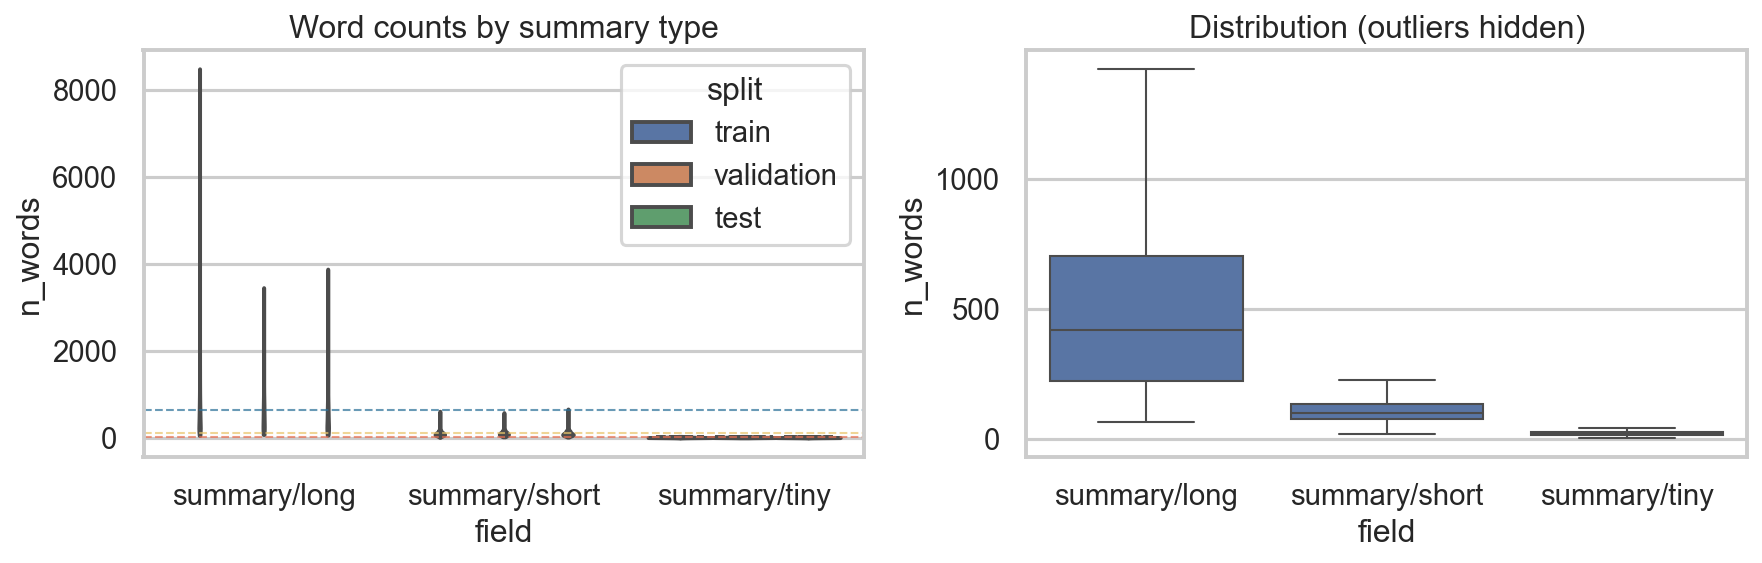
\includegraphics[width=\linewidth]{summary_words_violin.png}
\caption{Expert summary word counts by granularity and split (left: violin with targets as dashed lines; right: boxplot with outliers hidden).}
\label{fig:summary-words}
\end{figure}

\paragraph{Reading Figure~\ref{fig:summary-words}.}
The left panel shows wide long-summary distributions with a heavy right tail (test maximum 3{,}883 words), while short and tiny clusters near their dashed target lines. The right panel confirms that central mass for long summaries sits below the 650-word target even after hiding outliers. Splits behave similarly, so length skew is corpus-wide.

\paragraph{Design implication.}
ROUGE evaluation against long references remains meaningful, but systems should not be judged solely by matching a nominal 650-word average. Extreme long targets also increase the opportunity for citation-bearing sentences, relevant to Module~B.

\section{Granularity Switching and Compression}
\label{sec:eda-granularity}

Switching the target granularity changes both usable-case counts and compression ratio (source words / summary words). On the training split, median compression for long summaries is approximately 58$\times$, compared with roughly 2{,}400$\times$ for tiny summaries.

\begin{figure}[!t]
\centering
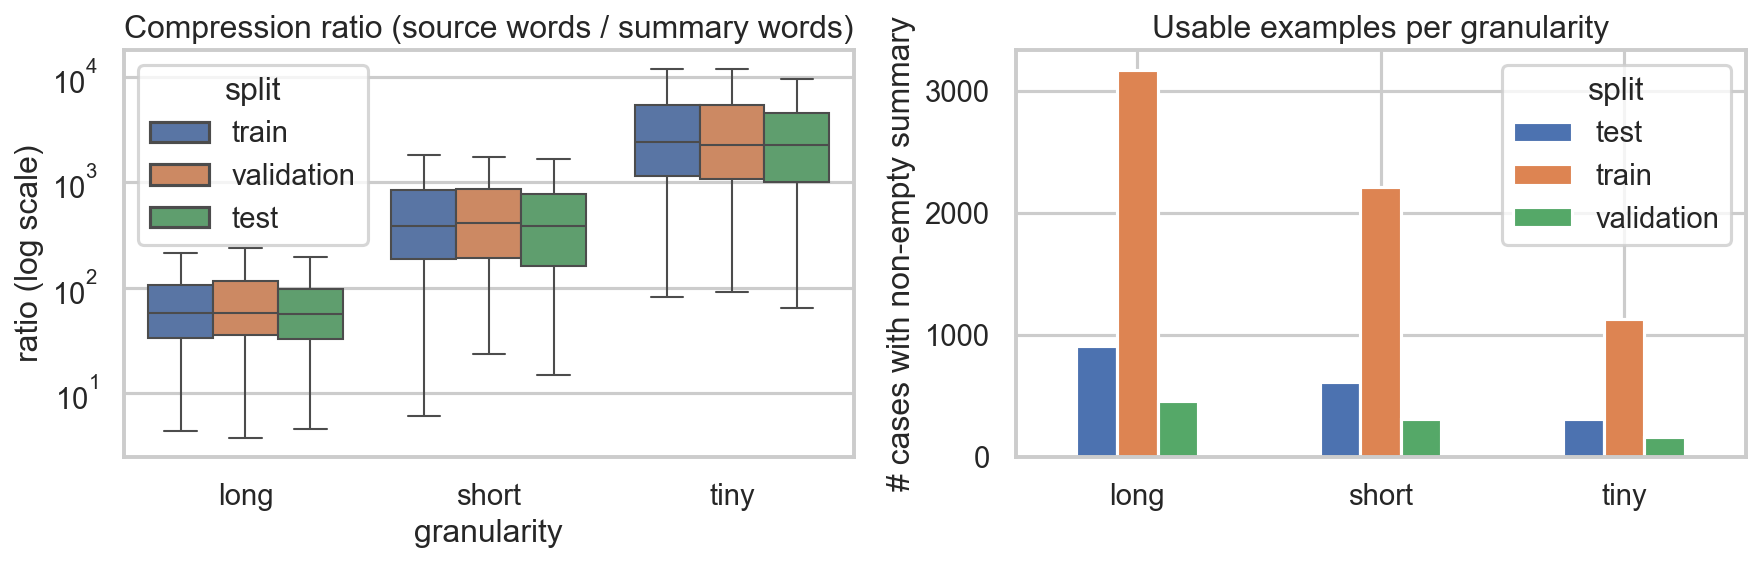
\includegraphics[width=\linewidth]{granularity_switch_analysis.png}
\caption{Left: compression ratio by granularity (log scale). Right: count of cases with non-empty expert summaries.}
\label{fig:granularity-switch}
\end{figure}

\paragraph{Reading Figure~\ref{fig:granularity-switch}.}
The left panel's log-scale boxes rise sharply from long to tiny, visualizing how aggressively each output word must compress the docket. The right panel restates availability: long bars dominate usable supervision. Together, the panels show that ``harder compression'' and ``fewer labels'' coincide at tiny granularity.

\paragraph{Design implication.}
Long summaries offer the richest context for citation extraction and verification; tiny summaries compress so aggressively that both modelling and citation auditing become less informative. This supports prioritizing $D\rightarrow L$ for RQ1--RQ3.

\section{Multi-Document Source Structure}
\label{sec:eda-sources}

Each case concatenates multiple legal documents. Corpus-wide source statistics are summarized in Table~\ref{tab:source-stats}. Mean source length (61{,}539 words) is consistent with the Multi-LexSum paper's long-docket narrative; the median (24{,}546 words) is lower, reflecting a heavy-tailed distribution.

\begin{table}[!t]
\centering
\caption{Per-case source statistics (all splits combined, $n=4{,}539$).}
\label{tab:source-stats}
\begin{tabular}{@{}l r r r@{}}
\toprule
\textbf{Statistic} & \textbf{Mean} & \textbf{Median} & \textbf{95th percentile} \\
\midrule
Source words        & 61{,}539 & 24{,}546 & 226{,}408 \\
Source characters   & 399{,}409 & 158{,}734 & 1{,}475{,}231 \\
\# source documents & 8.8 & 6.0 & 26.0 \\
\bottomrule
\end{tabular}
\end{table}

Approximately 35.1\% of cases include at least one OCR-derived source document.

\begin{figure}[!t]
\centering
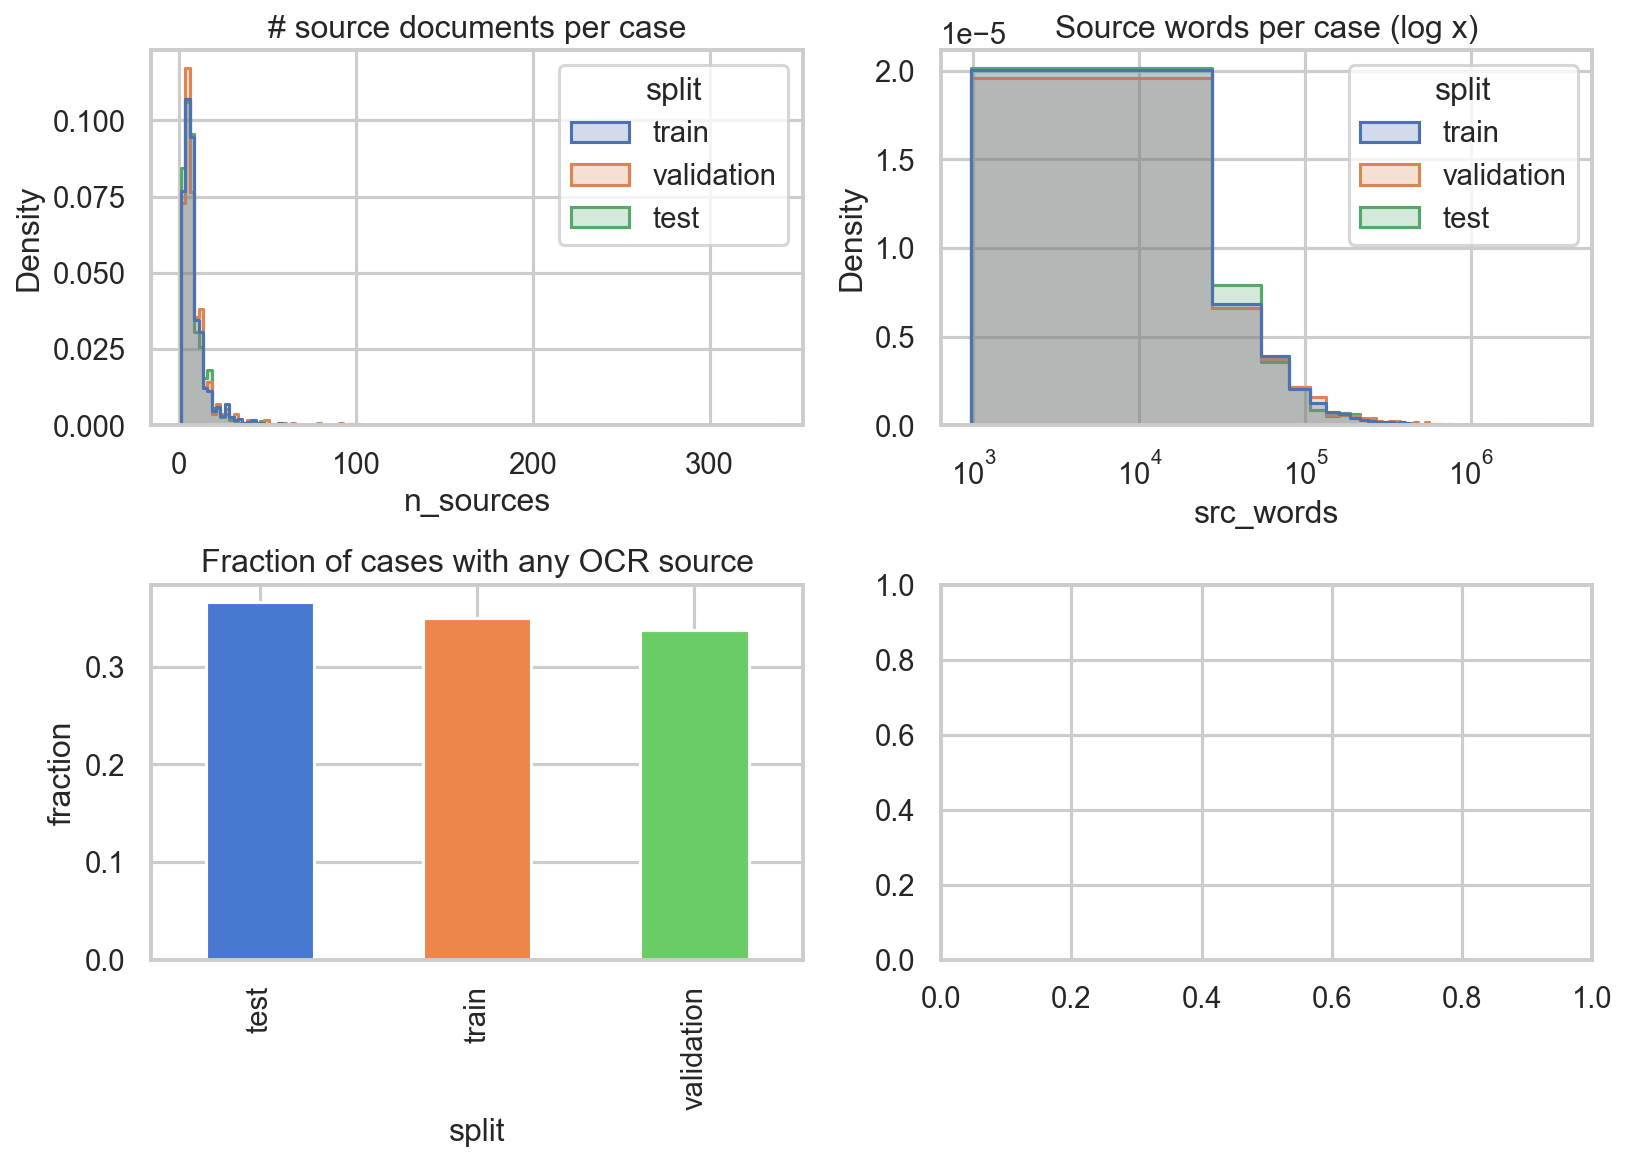
\includegraphics[width=0.88\linewidth]{source_distributions.png}
\caption{Per-case source document count (top left) and source word count on a log scale (top right). Bottom left: fraction of cases with any OCR source by split.}
\label{fig:source-distributions}
\end{figure}

\paragraph{Reading Figure~\ref{fig:source-distributions}.}
Document-count histograms peak at modest multi-document bundles but exhibit a long tail. Source-word histograms on a log axis show that ``typical'' cases are already tens of thousands of words, while a minority explode toward $10^5$--$10^6$ words. OCR prevalence near one-third warns that noisy text is common rather than exceptional.

\paragraph{Design implication.}
Module~A must assume heterogeneous, multi-file inputs. OCR noise can break brittle string matching, which is one reason Module~C reports Ambiguous/NotFound rather than forcing a match.

\section{Truncation Risk Under Fixed Context Budgets}
\label{sec:eda-truncation}

A GPT-2 tokenizer audit measures what fraction of cases exceed common token budgets (Table~\ref{tab:truncation}; training split).

\begin{table}[!t]
\centering
\caption{Fraction of training cases whose concatenated sources exceed a GPT-2 token budget.}
\label{tab:truncation}
\begin{tabular}{@{}r r@{}}
\toprule
\textbf{Token budget} & \textbf{Fraction exceeding} \\
\midrule
2{,}048    & 100.0\% \\
4{,}096    & 99.4\% \\
8{,}192    & 91.8\% \\
32{,}768   & 57.8\% \\
65{,}536   & 38.9\% \\
131{,}072  & 14.4\% \\
\bottomrule
\end{tabular}
\end{table}

\begin{figure}[!t]
\centering
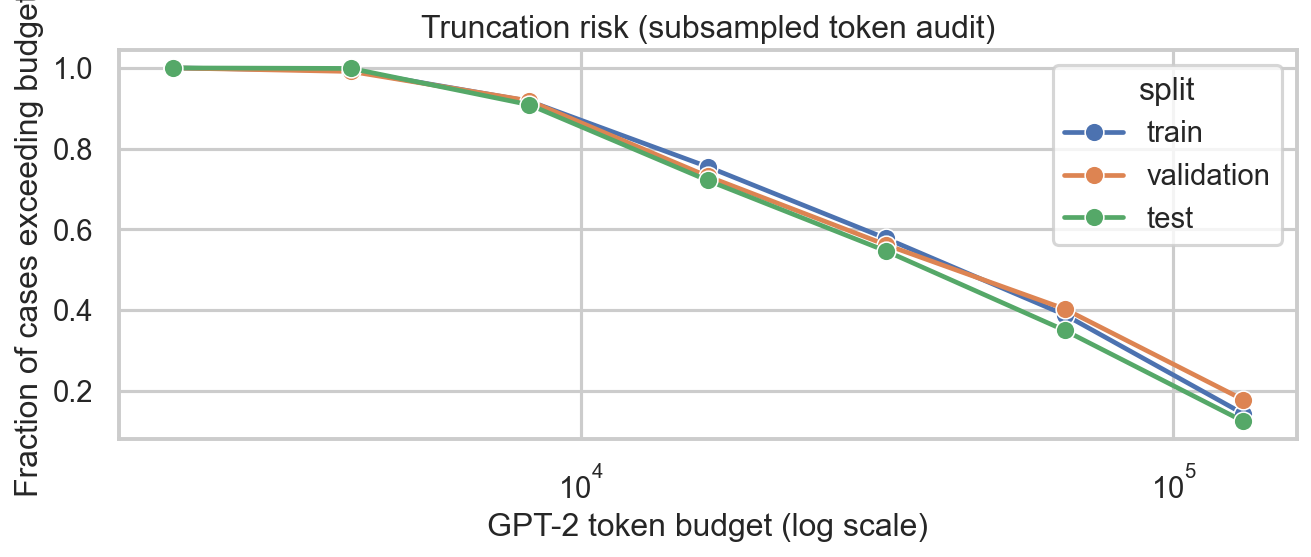
\includegraphics[width=0.88\linewidth]{truncation_fractions.png}
\caption{Fraction of cases exceeding a GPT-2 token budget across splits (log-scaled budgets on the $x$-axis).}
\label{fig:truncation}
\end{figure}

\paragraph{Reading Figure~\ref{fig:truncation}.}
All splits decay similarly: almost every case exceeds small budgets; a majority still exceed 32k tokens; a non-trivial fraction remains over budget even at 131k. The curve is the empirical argument against pretending Module~A ``reads the whole case.''

\paragraph{Design implication.}
Faithful summarization and citation verification must assume partial observability of the source. The dual-system design therefore treats the neural summarizer as an untrusted draft generator whose outputs are audited symbolically \cite{maynez2020faithfulness,beltagy2020longformer}. The 4{,}096-token truncation used for the full-scale run is an explicit, documented constraint, not a hidden footnote.

\section{Case Types, Outcomes, and Filing Years}
\label{sec:eda-metadata}

Multi-LexSum cases are drawn from U.S.\ civil-rights litigation filed between 1951 and 2021. The most frequent case type is Equal Employment (1{,}579 cases), followed by Immigration and/or the Border (523) and Prison Conditions (424). Plaintiffs prevail in 3{,}143 cases; defendants in 564; outcomes are mixed or pending for the remainder. Class actions are sought in 1{,}510 cases (33.3\%).

\begin{figure}[!t]
\centering
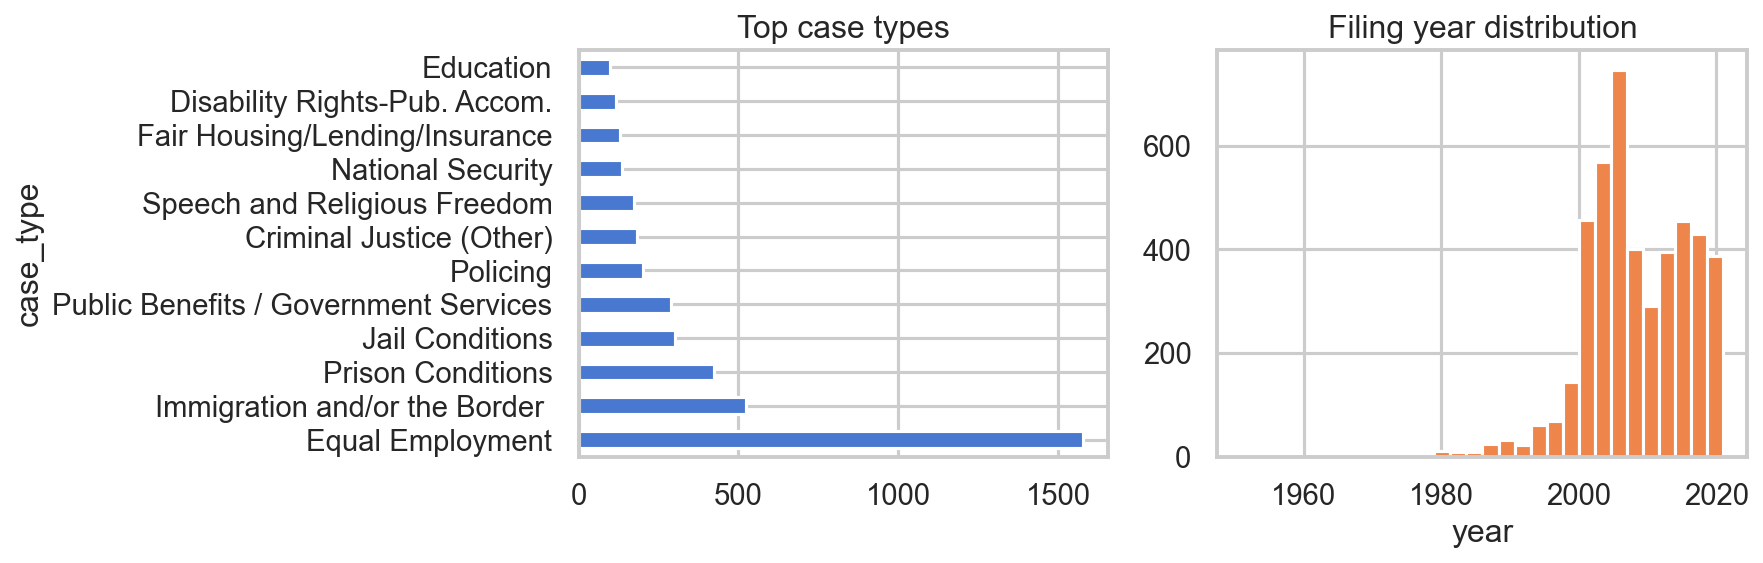
\includegraphics[width=\linewidth]{metadata_landscape.png}
\caption{Top case types (left) and filing-year distribution (right).}
\label{fig:metadata}
\end{figure}

\paragraph{Reading Figure~\ref{fig:metadata}.}
The left panel shows a skewed case-type distribution dominated by employment litigation, with a long tail of other civil-rights categories. The right panel shows filings spanning seven decades, concentrated in more recent decades but not confined to a single era. Domain diversity is real, but not uniform.

\paragraph{Design implication.}
Citation verification must handle heterogeneous reporters and eras. A single ``easy'' subset (e.g., only modern Supreme Court cites) would overstate verifier performance.

\section{Citation Density in Expert Summaries}
\label{sec:eda-citations}

Expert summaries provide a proxy for where citations appear in gold text. Regex heuristics (Federal Reporter patterns, \texttt{v.} party pairs) extract candidate spans, noisy but useful for relative comparisons across granularities.

\begin{table}[!t]
\centering
\caption{Heuristic citation statistics in expert summaries (train split, present summaries only).}
\label{tab:citation-density}
\begin{tabular}{@{}l r r r@{}}
\toprule
\textbf{Granularity} & \textbf{Mean hits} & \textbf{\% with $\geq 1$ hit} & \textbf{Mean cites / 100 words} \\
\midrule
Long  & 1.43 & 37.1\% & 0.20 \\
Short & 0.10 & 7.6\%  & 0.07 \\
Tiny  & 0.02 & 2.1\%  & 0.12 \\
\bottomrule
\end{tabular}
\end{table}

\begin{figure}[!t]
\centering
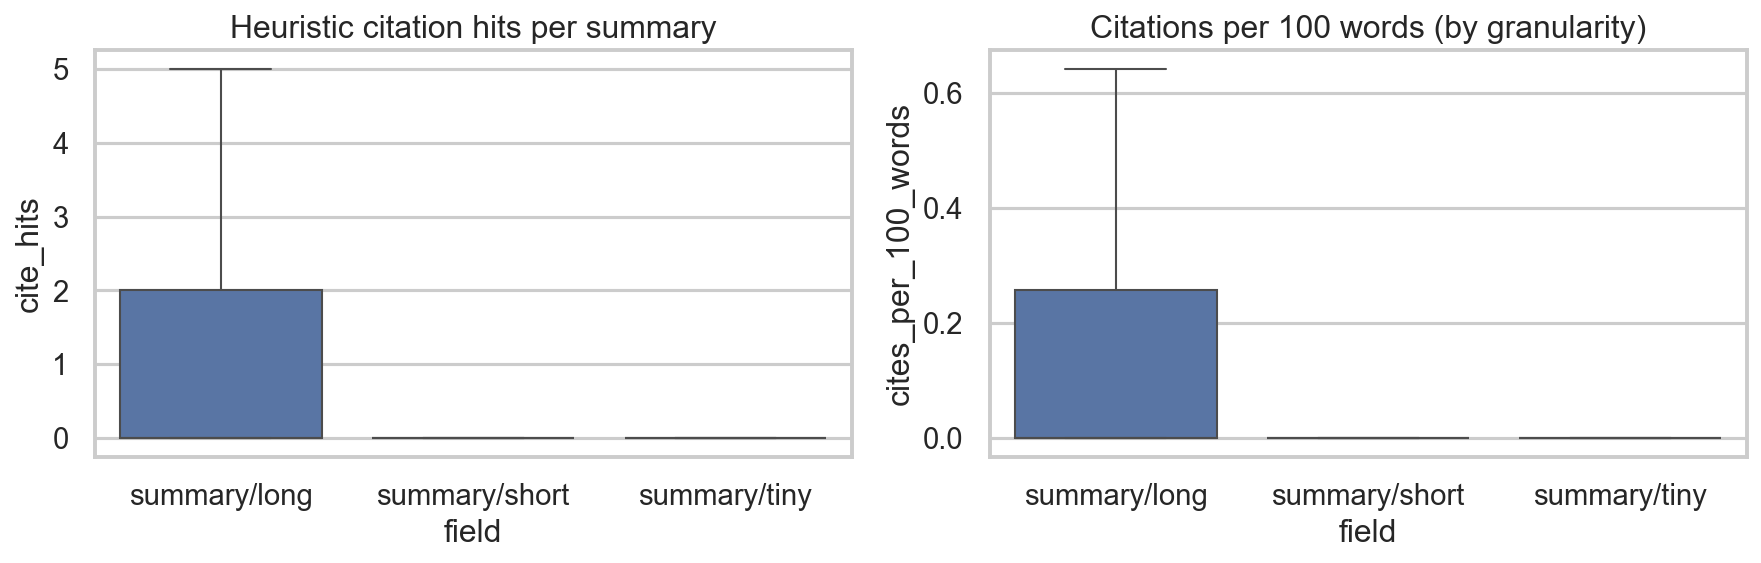
\includegraphics[width=\linewidth]{citation_by_granularity.png}
\caption{Heuristic citation hits (left) and citations per 100 words (right) by summary granularity.}
\label{fig:citation-granularity}
\end{figure}

\paragraph{Reading Figure~\ref{fig:citation-granularity}.}
Long summaries dominate absolute hit counts: most mass sits at zero, but the upper quartile carries multiple hits. Short and tiny summaries rarely contain heuristic cites. Normalized density (right) remains highest for long targets in absolute opportunity for Module~B, even though per-100-word rates can look noisy at tiny lengths due to short denominators.

\paragraph{Design implication.}
Citation verification is most informative at the long granularity. Module~B therefore targets $D\rightarrow L$ outputs; regex EDA is only a prior, and production extraction uses eyecite \cite{eyecite2021}.

\section{Data Quality Checks}
\label{sec:eda-quality}

Automated anomaly checks found no empty long summaries, no empty source lists, and no zero-length source documents. Missing short and tiny summaries are dataset characteristics rather than corruption (Section~\ref{sec:eda-corpus-shape}). The EDA pipeline exports \texttt{sample\_indices.csv} for stratified manual review; per license constraints, raw summary text from the audit subset remains internal to coursework.

\section{Summary of EDA Findings}
\label{sec:eda-summary}

The EDA supports four design decisions for the remainder of the thesis:
\begin{enumerate}
  \item \textbf{Primary task:} $D\rightarrow L$, where all splits have complete labels and citation opportunity is highest.
  \item \textbf{Modeling constraint:} truncation/chunking is unavoidable for most cases; faithfulness cannot rely on full-source attention alone.
  \item \textbf{Verification focus:} case-citation checking targets long outputs; short/tiny ablations are secondary.
  \item \textbf{Baseline expectations:} expert summaries already show moderate deviation from nominal length targets and sparse citation patterns under regex mining; automatic systems face a difficult faithfulness ceiling even before hallucination is measured on model outputs.
\end{enumerate}

These findings do not yet answer RQ1--RQ3, which require generated summaries from Module~A. They establish the empirical context in which the dual-system pipeline of Chapter~\ref{ch:methodology} is designed.
